% 2010 年浙江卷文科第 17 题：平行四边形 ABCD，O 为对角线交点，
% P、Q、M、N 分别为 OA、OB、OC、OD 的中点。
% 来源 PDF：普通高考/2010/2010浙江文.pdf，SHA-256 a73e22ea405697775b2d5cd82532fcffad0f506b849d9f199265b4297b8a754b。
% 原页：第 1 页（A3 三栏）第 3 栏中部，书页码 641。
% 重绘依据：照原页，A 左上、B 右上、D 左下、C 右下；对角线 AC、BD 交于 O；
%   P 在 OA 上、Q 在 OB 上、M 在 OC 上、N 在 OD 上，四点均以实心点标出。
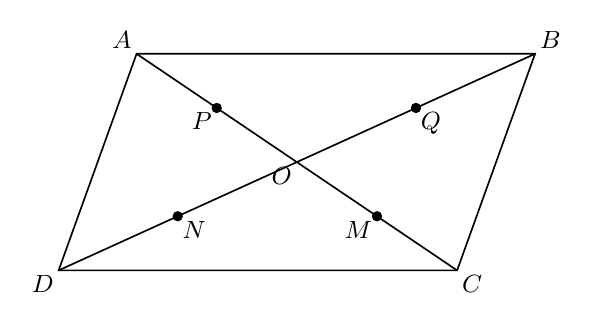
\begin{tikzpicture}[scale=1.1, semithick, every node/.style={inner sep=1.5pt, font=\small}]
  \coordinate (A) at (0.9,3.1);
  \coordinate (B) at (5.5,3.1);
  \coordinate (C) at (4.6,0.6);
  \coordinate (D) at (0,0.6);
  \coordinate (O) at (2.75,1.85);
  \coordinate (P) at (1.825,2.475);
  \coordinate (Q) at (4.125,2.475);
  \coordinate (M) at (3.675,1.225);
  \coordinate (N) at (1.375,1.225);

  \draw (A) -- (B) -- (C) -- (D) -- cycle;
  \draw (A) -- (C);
  \draw (B) -- (D);

  \fill (P) circle (1.7pt);
  \fill (Q) circle (1.7pt);
  \fill (M) circle (1.7pt);
  \fill (N) circle (1.7pt);

  \node[above left] at (A) {$A$};
  \node[above right] at (B) {$B$};
  \node[below right] at (C) {$C$};
  \node[below left] at (D) {$D$};
  \node[below left] at (O) {$O$};
  \node[below left] at (P) {$P$};
  \node[below right] at (Q) {$Q$};
  \node[below left] at (M) {$M$};
  \node[below right] at (N) {$N$};
\end{tikzpicture}
